\section{Rút trích đặc trưng}
Với các bài toán giải quyết bằng phương pháp học máy, bước trích xuất đặc trưng là quan trọng nhất. Bước này định nghĩa những đặc trưng nào được sử dụng và sử dụng như thế nào. Chúng tôi xem xét 4 đặc trưng sau: n-gram, change phrase, negation và so-cal. Trong phần này, mỗi mục con trình bày theo thứ tự: ...
\subsection{Tiền xử lý dữ liệu} \label{sec:tien-xu-ly}
Đây là bước xử lý trước khi có thể rút trích đặc trưng. Trong bước này, chúng tôi xử lý dữ liệu theo thứ tự:
\begin{itemize}
\item[•] Tách câu: Từ dữ liệu thu thập được, chúng tôi cần tách thành các câu. Tách một đoạn văn thành câu có thể dựa vào các dấu câu như dấu chấm (.) hoặc dấu 2 chấm (:), \ldots
\item[•] Chuyển tất cả các ký tự thành chữ thường.
\item[•] Xóa các ký tự đặc biệt, gồm: ?, \%, @, \#, $\wedge$, \$, ., ,,  ;, :, /, ", (, ), +, -, =
\item[•] Thay tất cả số bằng nhãn \term{DIGIT}.
\item[•] Loại bỏ \term{Stop words}: Các từ \term{stop word} là những từ thông thường được sử dụng mà có tính chất phân cực thấp. Một số từ \term{stop word} như: it, I, you, then, \ldots
\item[•] \term{Tokenization}: Sử dụng ký tự khoảng trắng để tách tách câu thành các token
\item[•] \term{Lemmatization:} Trả về dạng đúng của một động từ, dù động từ đó đang ở thì nào. \term{Lemmatization} thực hiện bằng cách loại bỏ đi các biến tố (\term{inflectional}). \\
Ví dụ: ``produced'' -> ``produce''.
\item[•] \term{Stemming} Loại bỏ hầu hết các hậu tố của 1 từ, trả về gốc của một từ dù từ đó được dùng như động từ, tính từ, danh từ hay phó từ.\\
 Ví dụ:  ``produced'' hoặc ``production'' -> ``produc''.
\end{itemize}

\subsection{N-gram} \label{subsec:ngram}
Giải thuật trích xuất đặc trưng n-gram trải qua 2 bước, được mô tả như Hình \ref{fig:mo-hinh-ngram}\\
\begin{figure}[h]
\centering
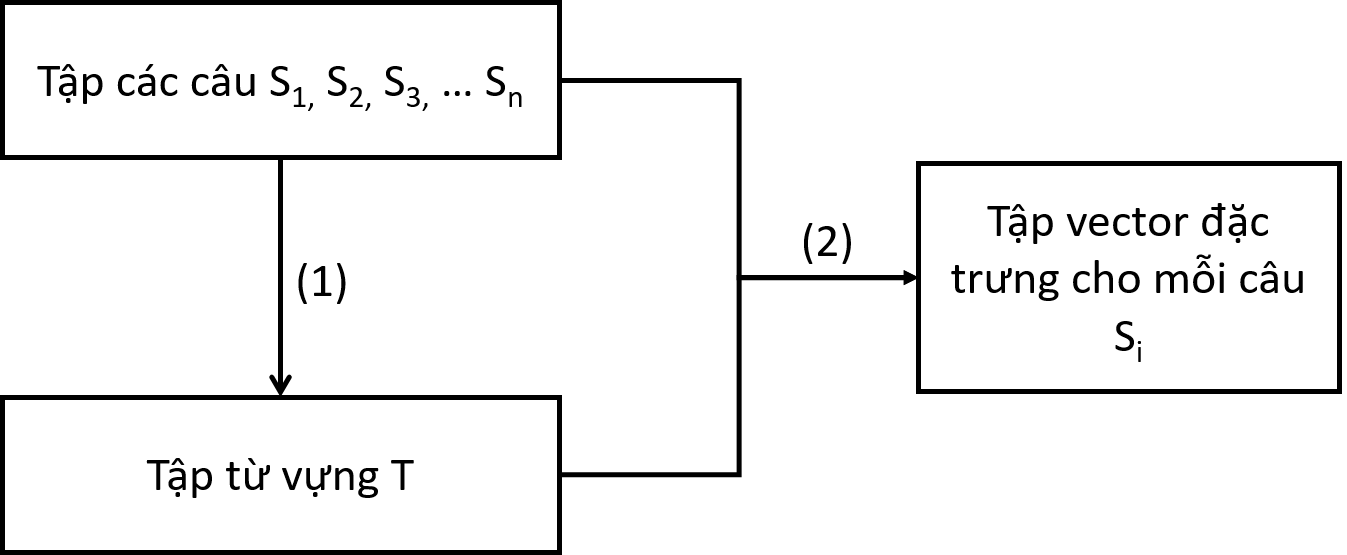
\includegraphics[scale=0.30]{../hinh/mo-hinh-ngram.png}
\caption{Giải thuật trích xuất đặc trưng n-gram} \label{fig:mo-hinh-ngram}
\end{figure}

Ở bước đầu tiên (1), giải thuật nhận vào tập hợp các câu. Mỗi câu sẽ được tách ra thành các n-gram. Tất cả các n-gram từ các câu sẽ được tổng hợp lại thành tập từ vựng T. Tuy nhiên, không phải tất cả các n-gram đều được thêm vào tập từ vựng T. Giải thuật quy định 1 mức ngưỡng $min\_df$ là số câu tối thiểu cùng chứa 1 n-gram thì n-gram đó mới được thêm vào tập T. Nếu $min\_df=1$ thì tập từ vựng T chứa tất cả các n-gram. Nghiên cứu \cite{sarker2011outcome} sử dụng $min\_df = 5$, trong khi nghiên cứu \cite{niu2005analysis} dùng $min\_df=4$. Tuy nhiên cả 2 nghiên cứu trên đều không giải thích về cách chọn các giá trị trên. Trong nghiên cứu này, chúng tôi tiến hành các thí nghiệm để phân tích và chọn ra giá trị $min\_df$ tối ưu nhất.\\

Bước còn lại là vector hóa câu: chuyển 1 câu từ dạng \term{text} sang dạng vector đại diện cho câu đó. Đầu tiền, cần sắp xếp các n-gram trong tập từ vựng T ở bước (1). Việc sắp xếp này là tùy ý, nhưng sau khi đã sắp xếp phải giữ nguyên thứ tự các n-gram trong tập T. Giả sử $T=\{\text{n-gram}_1, \text{n-gram}_2, \text{n-gram}_3, \ldots, \text{n-gram}_n\}$. Khi đó, mỗi câu $s_i$ sẽ được chuyển thành vector $v_i$ có n chiều. Có 2 cách hiện thực để xác định giá trị tại chiều thứ $k$ của vector $v_i$
\begin{enumerate}
\item Giá trị tại chiều thứ $k$ của vector $v_i$ là giá trị nhị phân, bằng 0 nếu câu đó không chứa $\text{n-gram}_k$, bằng 1 nếu câu đó chứa $\text{n-gram}_k$.
\item Giá trị tại chiều thứ $k$ của vector $v_i$ là số nguyên, thể hiện số lần xuất hiện $\text{n-gram}_k$ trong câu đó.
\end{enumerate}
Để thuận tiện khi gọi tên trong các thử nghiệm, chúng tôi quy ước đặt tên cách hiện thực thứ nhất là \term{vector nhị phân}, cách hiện thực thứ 2 là \term{vector số nguyên}. \\
\example{3}{
Giả sử sau khi qua bước (1), thu được tập từ vựng T gồm các n-gram như sau: drug, risk, disturbances, associated with, disadvantage, evidence. Khi đó, nếu sử dụng cách vector hóa dùng \term{vector nhị phân}, các câu ở ví dụ 1 và 2 được chuyển thành dạng vector như sau:
}
\begin{tabular}{| c | c | c | c | c | c | c | c |}
\hline
  & \textbf{drug} & \textbf{risk} & \textbf{disturbances} & \textbf{associated with} & \textbf{disadvantage} & \textbf{evidence}
\\ \hline
Ví dụ 1 & 0 & 1 & 0 & 1 & 0 & 0
\\ \hline
Ví dụ 2 & 0 & 1 & 0 & 0 & 1 & 0
\\ \hline
\end{tabular}
Khi đó, $v_1 = (0, 1, 0, 1, 0, 0) $ và $v_2=(0, 1, 0, 0, 1, 0)$
\subsection{Change phrase}
Rút trích đặc trưng Change phrase phụ thuộc vào 2 yếu tố:
\begin{itemize}
\item[•] Danh sách từ trong mỗi nhóm LESS, MORE, BAD, GOOD
\item[•] Giải thuật nhận biết sự kết hợp của các nhãn trên
\end{itemize}
Với yếu tố thứ nhất, trong nghiên cứu này, chúng tôi sử dụng danh sách từ cho mỗi nhóm tham khảo từ nghiên cứu của nhóm tác giả Sarker, Abeed, et al.\cite{sarker2011outcome}. Nhóm tác giả trên tự tập hợp danh sách các nhóm từ thủ công nhưng không liệt kê trong báo cáo của mình. Nhóm chúng tôi có liên hệ và đã nhận được mã nguồn, từ đó lấy được danh sách các nhóm từ. Danh sách này gồm 371 từ (BAD: 223 từ, GOOD: 82 từ, MORE: 30 từ, LESS:36 từ). Sau đó, chúng tôi mở rộng danh sách bằng cách thu thập thủ công. Danh sách cuối cùng gồm 423 từ (BAD: 238, GOOD: 96, MORE: 42 từ, LESS: 47 từ).\\

Sau khi đã có tập hợp các từ cho mỗi nhóm, chúng tôi xem xét yếu tố thứ 2: hiện thực giải thuật nhận dạng xem 1 câu có thuộc mẫu nào trong 4 mẫu: LESS-GOOD, LESS-BAD, MORE-GOOD, MORE-BAD. Giải thuật nhận dạng câu thuộc mẫu nào được thực hiện qua 2 bước.\\

Ở bước 1, giải thuật nhận dạng những từ mô tả sự thay đổi, bằng cách so trùng các từ trong 2 nhóm LESS và MORE với các từ trong câu. Để có thể so trùng thành công, trước tiên các từ trong 2 nhóm này được xử lý \term{lemmatization} và \term{stemming} như ở mục \ref{sec:tien-xu-ly}. Sau đó mỗi từ trong câu được so sánh với các từ trong 2 nhóm trên. Nếu từ $w$ thuộc 1 trong 2 nhóm trên, giải thuật thêm \term{tag} ``\_LESS'' hoặc ``\_MORE'' vào cuối các từ thuộc phạm vi từ từ $w$ đến dấu chấm câu gần nhất (về phía cuối câu). Dấu chấm câu có thể là dấu chấm (.), dấu phẩy (,), dấu hai chấm (:) hoặc dấu chấm phẩy (;).\\

\example{1}{\myquote{Atypical antipsychotic use is associated with an increased risk for death compared with nonuse among older adults with dementia}. Giải thuật sẽ đánh dấu \term{tag} ``\_MORE'' từ từ increased đến hến câu: ``Atypical antipsychotic use is associated with an increased risk\_MORE for\_MORE death\_MORE compared\_MORE with\_MORE nonuse\_MORE among\_MORE older\_MORE adults\_MORE with\_MORE dementia\_MORE''. Ở bước này, đặc trưng Change phrase không thực sự tạo ra một đặc trưng mới, nó chỉ làm thay đổi các n-gram: từ risk thành rish\_MORE, từ đó thay đổi đặc trưng n-gram. Bằng cách này, thông qua đặc trưng n-gram, Change phrase không chỉ nhận biết được trong câu có sự mô tả về thay đổi, mà còn biết được phạm vi ảnh hưởng của sự thay đổi đó.}

Bước 2 nhận diện xem câu có thuộc mẫu nào trong 4 mẫu: LESS GOOD, LESS BAD, MORE GOOD, MORE BAD hay không. Nếu trong câu có 1 từ thuộc nhóm MORE, giải thuật sẽ xác định trong phạm vi từ từ đó đến hết câu, nếu có từ nào thuộc nhóm GOOD, câu đó thuộc mẫu MORE-GOOD. Tương tự như vậy đối với 3 mẫu còn lại.

\subsection{Yếu tố phủ định}
\subsubsection*{Tổng quan}
%Định nghĩa
Yếu tố phủ định (negation) là một từ hoặc cụm từ mang ý nghĩa phủ nhận sự tồn tại của một yếu tố khác trong câu \cite{skeppstedt2016marker}. Cụ thể trong bài toán phân loại cảm xúc, ở câu "He denies any antecedent palpitations, shortness of breath, chest pain, headache, or lightheadedness", yếu tố phủ định được xác định là "denies" phủ nhận sự tồn tại của một loạt các triệu chứng bệnh "palpitations", "shortness of breath", "chest pain", "headache", "lightheadedness".  \\

Nhiều thuật toán phân tích phủ định đã được hiện thực trên văn bản tiếng Anh (2-5)\cite{Chapman2013}, \cite{Zeng2007} và một số trong đó được phát triển để nhận diện phủ định cho các ngôn ngữ khác \cite{costumero2014an}, \cite{benamara2012how}, \cite{gindl2006negation}, \cite{Chapman2013}, \cite{CruzDiaz2015}. \\

%Negation bao gồm các thành phần chính....

%Lợi ích
Trong lĩnh vực nghiên cứu về xử lý ngôn ngữ tự nhiên nói chung và trong bài toán phân tích cảm xúc nói riêng, việc xử lý phủ định //mang lại lợi ích... \\
\cite{liu2012sentiment}\cite{marsland2015machine}\cite{Giachanou2016}\cite{ali2013can}\cite{taboada2011lexicon}\cite{niu2006using}\cite{ohana2009sentiment}

\subsection{SO-CAL}
